\chapter{Il percorso di ricerca: ipotesi testate e scartate}
\label{ch:percorso}

La strategia presentata in questa tesi è il risultato di un processo di
eliminazione. Prima di arrivare alla selezione Top Vega descritta nel
Capitolo~\ref{ch:strategia}, sono state costruite e testate cinque ipotesi
progressivamente più sofisticate, ciascuna scartata sulla base di un
criterio quantitativo esplicito. Documentare questo percorso, e non solo
l'esito, risponde a una precisa scelta metodologica: la letteratura sulle
strategie di trading è affetta da un marcato \emph{publication bias}, che
premia i risultati positivi e nasconde i tentativi falliti. Rendere
espliciti gli insuccessi ha due vantaggi. Da un lato, mostra che la
semplicità della strategia finale non è ingenuità ma il residuo di un
vaglio severo. Dall'altro, alcuni degli insuccessi (in particolare
l'artefatto documentato nella \S\ref{sec:percorso-premium-dte}) sono
lezioni metodologiche di portata generale per chiunque backtesti strategie
in opzioni su strumenti illiquidi.

\section{Ipotesi 1: il gap RND--KDE come segnale di selezione}
\label{sec:percorso-rnd-kde}

La prima ipotesi nasceva dall'idea più naturale in un contesto di vendita
di volatilità: se il premio esiste perché la densità risk-neutral
sovrastima la probabilità degli eventi estremi rispetto alla densità
fisica, allora il divario \emph{pointwise} tra le due densità dovrebbe
identificare le opzioni più sopravvalutate. Il punteggio assegnato a
ciascuna opzione era il prodotto tra il gap di probabilità (RND meno densità
fisica al relativo strike) e il vega dell'opzione, così da pesare il segnale
per la sensibilità alla volatilità. L'infrastruttura completa (segnale,
esecuzione, copertura, uscita, audit) è stata costruita con tempistica T+1 e
sottoposta a una griglia di sensibilità $6\times 5$, con celle tutte
profittevoli sia in-sample sia out-of-sample.

Il risultato apparentemente incoraggiante nascondeva però un problema di
fondo, emerso dal test critico. Non è sufficiente che il gap sia positivo
in media: il gap grezzo \emph{è} il premio per il rischio di volatilità, ed
è positivo quasi sempre proprio perché la volatilità implicita eccede
quella realizzata. Verificare che il gap grezzo sia positivo risponde alla
domanda banale, se il VRP esista, non alla domanda rilevante, se il segnale
sappia \emph{discriminare} i momenti e gli strumenti in cui vendere è più
conveniente. Per isolare la seconda domanda, il gap è stato reso a media
nulla (demeaned) tramite una media espansiva, strettamente causale, e
regredito sul profitto realizzato per trade con errori standard raggruppati
per data. Il coefficiente stimato è risultato negativo e non
significativo ($\beta < 0$, $p = 0{,}37$): il segnale, una volta rimossa la
componente banale, non ha alcun potere predittivo sul profitto dei singoli
trade. A conferma, un semplice benchmark che seleziona l'opzione a vega
massimo batteva la strategia complessa con meno trade e uno Sharpe
superiore.

La diagnosi è che il confronto pointwise tra due densità entrambe stimate
con errore produce un segnale dominato dal rumore. La densità fisica stimata
via kernel density estimation, sotto ipotesi di rendimenti indipendenti e
identicamente distribuiti su una finestra di 365 giorni, è troppo imprecisa
sulle code, proprio dove il gap dovrebbe essere informativo. Il gap è stato
dunque abbandonato come segnale di selezione, mentre la densità risk-neutral
è rimasta come infrastruttura tecnica e strumento di analisi.

\section{Ipotesi 2: la selezione Premium/DTE e l'artefatto bid=0}
\label{sec:percorso-premium-dte}

La seconda ipotesi puntava a massimizzare l'efficienza del premio per unità
di tempo, selezionando l'opzione con il rapporto più elevato tra premio
incassato e giorni alla scadenza (bid $\times$ spot / DTE). I risultati
iniziali erano notevoli: uno Sharpe in-sample di 1,67 su 126 trade, e una
correlazione quasi nulla con la selezione Top Vega, tale da suggerire un
portafoglio diversificato tra le due.

L'audit ha rivelato che l'intera redditività era un artefatto. Il problema
critico riguardava le opzioni profondamente in-the-money, che lo scoring
privilegiava perché caratterizzate da premi elevati (il delta mediano dei
trade selezionati era 0,99). Su Deribit queste opzioni sono di fatto
illiquide: nessun operatore le quota in acquisto, e il loro \emph{bid} nei
dati risulta pari a zero. Il backtest osservava quindi un prezzo di uscita
nullo, interpretava la posizione come chiusa avendo catturato il 100\% del
premio, e registrava un profitto inesistente. La
Tabella~\ref{tab:premium-dte-artefatto} scompone il fenomeno: 33 dei 126
trade (il 26\%) avevano prezzo di uscita nullo e generavano da soli 351.000
dollari, pari al 116,6\% del profitto totale di 301.000 dollari; i restanti
93 trade perdevano complessivamente 50.000 dollari. Senza l'artefatto, la
strategia era in perdita.

\begin{table}[H]
\centering
\caption{Scomposizione del profitto della strategia Premium/DTE (in-sample):
i trade con prezzo di uscita nullo, dovuti a opzioni illiquide, generano
oltre il 100\% dei profitti apparenti.}
\label{tab:premium-dte-artefatto}
\begin{tabular}{lcc}
\toprule
\textbf{Sottoinsieme di trade} & \textbf{Numero} & \textbf{Profitto aggregato} \\
\midrule
Trade con exit price $=0$ (illiquidi) & 33 & $+\$351.000$ \\
Trade con exit price $>0$ & 93 & $-\$50.000$ \\
\midrule
Totale apparente & 126 & $+\$301.000$ \\
\bottomrule
\end{tabular}
\end{table}

L'audit ha inoltre identificato due distorsioni minori ma sistematiche: le
uscite erano valorizzate al bid anziché all'ask (quando si riacquista
un'opzione corta si paga l'ask), e le opzioni non scontavano alcuna
commissione. Corretti tutti e tre i problemi (filtro sul delta $|\Delta| \le
0{,}50$ per escludere le opzioni deep in-the-money illiquide, uscita
all'ask, commissioni Deribit), lo Sharpe in-sample crollava a $-0{,}24$: la
strategia era morta.

Vale la pena notare che la prima interpretazione dell'anomalia era errata.
Si era ipotizzato che Premium/DTE fosse implicitamente una scommessa
direzionale, perché selezionava opzioni profondamente in-the-money. Ma se la
copertura delta funziona, anche un'opzione deep in-the-money è
delta-neutrale; il vero problema non era la direzionalità, bensì il prezzo
nullo nei dati. La diagnosi corretta è emersa solo scomponendo il profitto
dei singoli mega-trade, un promemoria del fatto che, nel backtesting di
strategie in opzioni, l'analisi aggregata può occultare artefatti che solo
l'ispezione trade per trade rivela.

\section{Ipotesi 3: multi-posizione per ampliare il campione}
\label{sec:percorso-multiposizione}

Una limitazione strutturale della strategia Top Vega è la bassa numerosità
campionaria: circa 35 trade in-sample in poco più di 800 giorni di
negoziazione. L'indagine ha mostrato che ciò non dipende da una scarsità di
segnali, ma dal lungo periodo di detenzione (DTE mediano all'ingresso di 66
giorni, holding medio di 25,5 giorni) combinato con il vincolo di posizione
singola: la strategia è di fatto investita per il 92,8\% del tempo (solo 61
giorni piatti su 851). Il problema non è la frequenza dei segnali, ma la
capacità di sfruttarli.

L'ipotesi naturale era allora consentire fino a tre posizioni simultanee,
diversificate per fascia di scadenza. La
Tabella~\ref{tab:multi-position} ne riporta i risultati.

\begin{table}[H]
\centering
\caption{Confronto tra posizione singola e multi-posizione (fino a 3
posizioni simultanee, diversificate per scadenza).}
\label{tab:multi-position}
\begin{tabular}{lcccc}
\toprule
\textbf{Metrica} & \textbf{Single IS} & \textbf{Multi IS} & \textbf{Single OOS} & \textbf{Multi OOS} \\
\midrule
Trade    & 35      & 147     & 10      & 60 \\
Sharpe   & 1,74    & 0,63    & 1,53    & 1,76 \\
Return   & 37\%    & 33\%    & 14\%    & 37\% \\
MTM DD   & $-18{,}4\%$ & $-49{,}7\%$ & $-4{,}5\%$ & $-14{,}5\%$ \\
\bottomrule
\end{tabular}
\end{table}

Il risultato è istruttivo perché la multi-posizione funziona nel periodo
out-of-sample (mercato calmo e rialzista) ma è devastante nel periodo
in-sample: il drawdown mark-to-market raggiunge il $-49{,}7\%$, contro il
$-18{,}4\%$ della posizione singola, con uno Sharpe che collassa da 1,74 a
0,63. La ragione è la correlazione: le posizioni parallele sono tutte corte
di volatilità sullo stesso sottostante, e durante un crash perdono
simultaneamente, mentre la copertura aggregata peggiora anziché migliorare.
La diversificazione per scadenza è illusoria quando il fattore di rischio
dominante, la volatilità di Bitcoin, è comune a tutte le posizioni. La
decisione è stata mantenere la posizione singola, accettando la bassa
frequenza come caratteristica intrinseca della strategia piuttosto che come
difetto da correggere.

\section{Filtri di regime: cinque indicatori senza potere predittivo}
\label{sec:percorso-regime}

L'analisi per regimi mostra che la strategia è forte in condizioni di
volatilità bassa e media e debole in alta volatilità, un profilo tipico
della vendita di volatilità. Ne discende l'ipotesi che un filtro capace di
ridurre l'esposizione, o di astenersi dal trading, nei momenti di alta
volatilità possa migliorare il rendimento corretto per il rischio. Per
verificarla, per ciascuno dei 35 trade in-sample è stato registrato il
valore di cinque indicatori al momento dell'ingresso, e ne è stata testata
la correlazione con il profitto del trade. La
Tabella~\ref{tab:regime-indicatori} riporta i risultati.

\begin{table}[H]
\centering
\caption{Indicatori di regime testati: correlazione con il profitto per
trade sui 35 trade in-sample. Nessun indicatore discrimina tra trade
vincenti e perdenti.}
\label{tab:regime-indicatori}
\begin{tabular}{lccc}
\toprule
\textbf{Indicatore} & \textbf{Corr. con PnL} & \textbf{Media winner} & \textbf{Media loser} \\
\midrule
DVOL (IV implicita)        & $+0{,}202$ & 76,4\%   & 74,6\% \\
Parkinson RV30             & $+0{,}237$ & 67,9\%   & 65,2\% \\
VRP spread (DVOL$-$RV30)   & $-0{,}133$ & 8,5 pp   & 9,4 pp \\
Skewness RND               & $-0{,}009$ & $-0{,}038$ & $-0{,}027$ \\
Curtosi RND                & $-0{,}086$ & 2,753    & 2,573 \\
\bottomrule
\end{tabular}
\end{table}

La scelta degli indicatori era economicamente motivata. Il DVOL misura il
livello della volatilità implicita, ossia quanto il mercato prezza la
volatilità futura; la RV30 di Parkinson misura il livello di volatilità
realizzata; lo spread tra i due è la misura più diretta del premio che si
sta vendendo, e concettualmente la più rilevante, perché se fosse invertito
(volatilità realizzata superiore all'implicita) non vi sarebbe premio da
catturare. La skewness e la curtosi della densità risk-neutral misurano
rispettivamente il rischio di coda e la pesantezza delle code prezzate dal
mercato.

Il risultato è che nessuno degli indicatori discrimina: tutte le
correlazioni sono in valore assoluto inferiori a 0,25, e le medie degli
indicatori nei trade vincenti e perdenti sono quasi indistinguibili.
Particolarmente istruttivo è il caso dello spread VRP, il candidato più
promettente in teoria: la sua correlazione con il profitto è addirittura di
segno negativo, e vi sono trade con spread molto elevato all'ingresso ($+12$
e $+31$ punti percentuali) che chiudono comunque in perdita. L'osservazione
di fondo è che il premio all'ingresso non è il fattore che determina il
profitto: quel che conta è ciò che accade \emph{durante} il trade, cioè se
sopraggiungano salti improvvisi o esplosioni di volatilità, eventi non
prevedibili dalle condizioni al momento dell'ingresso. Con soli 35 trade e
correlazioni tutte inferiori a 0,25, qualsiasi filtro costruito su questi
indicatori sarebbe privo di validità statistica. Nessun filtro di regime è
stato quindi implementato.

\section{Stop loss: un'analisi controfattuale}
\label{sec:percorso-stoploss}

L'ultima ipotesi riguardava lo stop loss. Una strategia short volatility
priva di stop è esposta, in linea di principio, a perdite di grande entità,
e la sua assenza richiede una giustificazione. L'analisi ha ricostruito, per
ciascuno dei 35 trade in-sample, il profitto mark-to-market non realizzato
giorno per giorno, registrando la perdita massima attraversata e
confrontandola con l'esito finale.

Tre osservazioni emergono. Primo, i trade vincenti attraversano
frequentemente drawdown significativi prima di recuperare: 15 dei 23
vincitori hanno registrato una perdita non realizzata inferiore a $-500$
dollari, e nel caso estremo un trade è sceso a $-17.386$ dollari (pari al
$-15{,}5\%$ del capitale) per poi chiudere a $+995$ dollari. Secondo, i
trade perdenti trascorrono molto più tempo in territorio negativo: in media
il 59\% dei giorni (15,1 giorni) contro il 29\% dei vincenti (6,2 giorni).
Terzo, sette trade erano in profitto oltre i 500 dollari prima di chiudere
in perdita, segno che il profit target non si è attivato in tempo.

Il test quantitativo, riportato nella Tabella~\ref{tab:stop-loss}, confronta
per ciascuna soglia di stop il profitto che sarebbe stato distrutto sui
trade vincenti stoppati prematuramente con quello che sarebbe stato
risparmiato sui trade perdenti.

\begin{table}[H]
\centering
\caption{Effetto controfattuale dello stop loss sui 35 trade in-sample. A
ogni soglia, il profitto distrutto sui trade vincenti supera quello
risparmiato sui perdenti.}
\label{tab:stop-loss}
\setlength{\tabcolsep}{6pt}
\begin{tabular}{lcccc}
\toprule
\textbf{Soglia} & \makecell{\textbf{Trade}\\\textbf{colpiti}} & \makecell{\textbf{di cui}\\\textbf{vincenti}} & \makecell{\textbf{PnL vincenti}\\\textbf{perso}} & \makecell{\textbf{PnL perdenti}\\\textbf{salvato}} \\
\midrule
$-1{,}0\%$ & 15 & 8 & \$23.380 & $-\$6.692$ \\
$-2{,}0\%$ & 5  & 3 & \$14.312 & $-\$2.928$ \\
$-3{,}0\%$ & 3  & 2 & \$8.619  & $-\$182$ \\
$-5{,}0\%$ & 2  & 2 & \$8.619  & \$0 \\
\bottomrule
\end{tabular}
\end{table}

\begin{figure}[H]
\centering
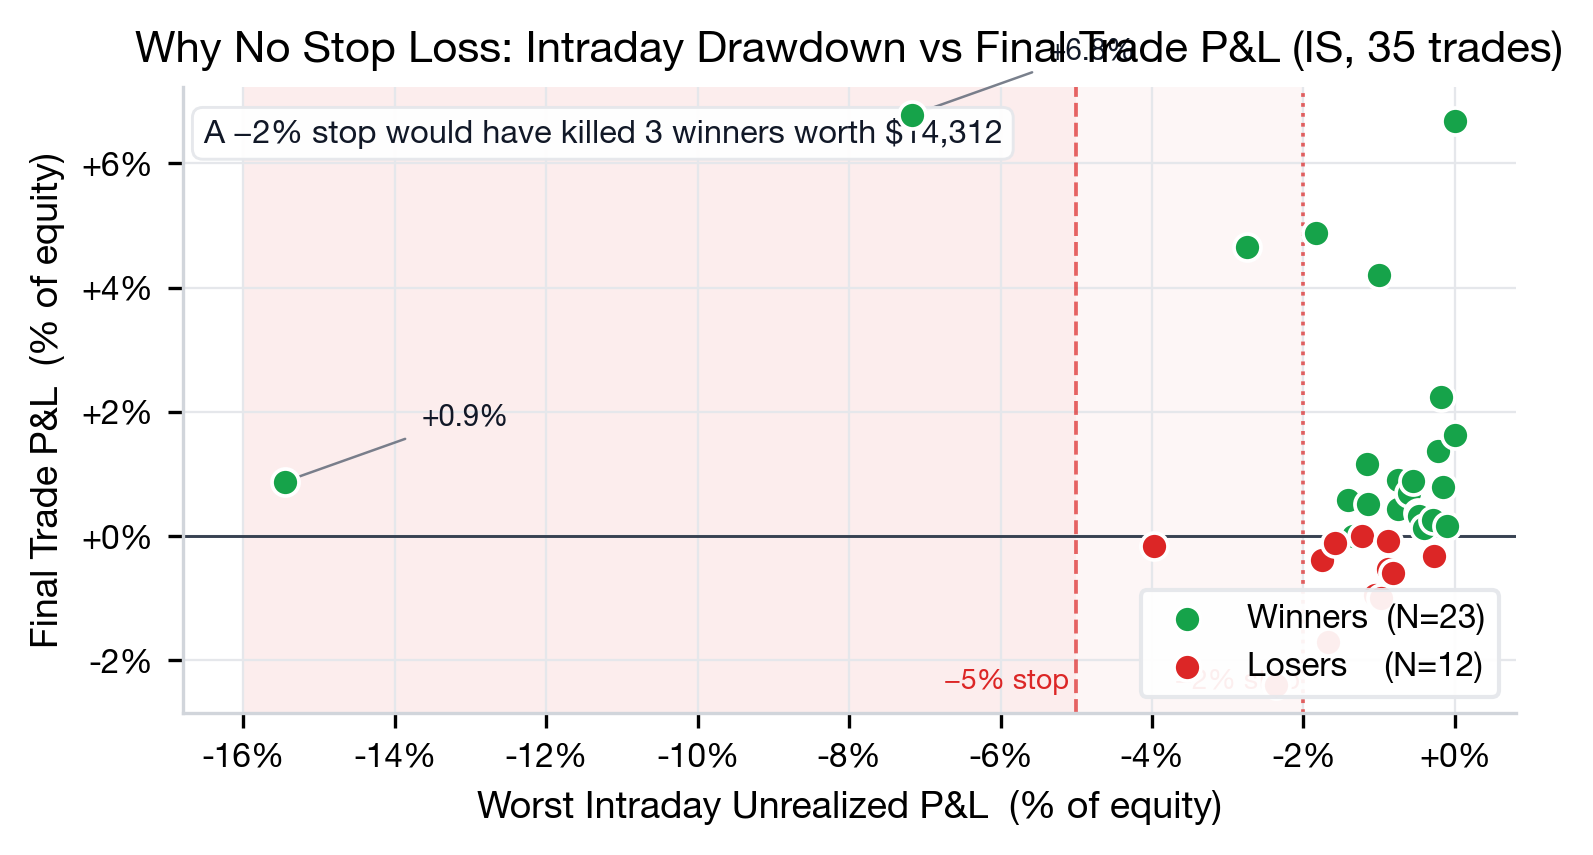
\includegraphics[width=\textwidth]{figures/fig3_stoploss.png}
\caption{Analisi dello stop loss: profitto distrutto sui trade vincenti
contro profitto risparmiato sui perdenti, per soglia di stop.}
\label{fig:stoploss}
\end{figure}

A ogni livello testato, il profitto perso sui vincenti stoppati supera
quello risparmiato sui perdenti; al di sotto del $-4\%$ verrebbero stoppati
soltanto trade vincenti. La spiegazione è economica: la strategia short
volatility genera profitto dal decadimento temporale (theta), che richiede
tempo per manifestarsi. Il profilo di payoff è asimmetrico nel tempo: la
perdita mark-to-market arriva subito, quando la volatilità implicita sale,
mentre il recupero è graduale e affidato al theta. Uno stop loss taglia
precisamente la fase di recupero, trasformando in perdite definitive
drawdown temporanei che si sarebbero riassorbiti. Nessuno stop loss è stato
quindi adottato: le uniche regole di uscita sono il profit target al 50\%
del premio e l'uscita temporale a 5 giorni dalla scadenza.

\section{Sintesi del processo di eliminazione}
\label{sec:percorso-sintesi}

La Tabella~\ref{tab:sintesi-decisioni} riepiloga le cinque ipotesi e il
criterio quantitativo che ha portato a scartarle. Il filo conduttore è che
ogni tentativo di aggiungere complessità, un segnale di selezione più
raffinato, un maggior numero di posizioni, un filtro di timing, una regola
di protezione, è stato sconfessato dai dati. La strategia sopravvissuta è la
più semplice tra quelle considerate, e la sua semplicità è il prodotto
diretto di questo vaglio, non una scelta di comodo.

\begin{table}[H]
\centering
\caption{Sintesi delle ipotesi testate e dei criteri di rigetto.}
\label{tab:sintesi-decisioni}
\small
\begin{tabular}{p{4.2cm}p{8.5cm}}
\toprule
\textbf{Ipotesi} & \textbf{Criterio di rigetto} \\
\midrule
Gap RND--KDE come segnale & $\beta < 0$, $p = 0{,}37$ sul gap demeaned regredito sul PnL; nessun potere predittivo \\
Selezione Premium/DTE & Il 116,6\% dei profitti era artefatto di prezzi di uscita nulli su opzioni illiquide; post-fix Sharpe $-0{,}24$ \\
Multi-posizione & Drawdown in-sample $-49{,}7\%$; le posizioni correlano nei crash \\
Filtri di regime & Cinque indicatori, tutte le correlazioni con il PnL inferiori a 0,25 \\
Stop loss & A ogni soglia distrugge più profitto sui vincenti di quanto ne salvi sui perdenti \\
\bottomrule
\end{tabular}
\end{table}
